\chapter{Analiza efektywności}
\thispagestyle{chapterBeginStyle}

\iffalse
W tym rozdziale należy omówić zawartość pakietu instalacyjnego oraz założenia co do środowiska, w którym realizowany system będzie instalowany. Należy przedstawić procedurę instalacji i wdrożenia systemu. Czynności instalacyjne powinny być szczegółowo rozpisane na kroki. Procedura wdrożenia powinna obejmować konfigurację platformy sprzętowej, OS (np. konfiguracje niezbędnych sterowników) oraz konfigurację wdrażanego systemu, m.in.\ tworzenia niezbędnych kont użytkowników. Procedura instalacji powinna prowadzić od stanu, w którym nie są zainstalowane żadne składniki systemu, do stanu w którym system jest gotowy do pracy i oczekuje na akcje typowego użytkownika.


Kompilator zawarty w programie służy do kompilowania programów i zapytań Prologa do instrukcji maszyny Warrena. Kompilator rozpoznaje czy na wejściu dostaje zapytanie czy program, po tym że zapytania zaczynają się od \texttt{?-}. Dla programu instrukcje generowane są dla każdej klauzuli osobno, a następnie łączone w ze sobą w całość. Nazwy struktur i zmiennych mogą zawierać wielkie i małe litery, cyfry i podkreślniki.\\
Kompilator akceptuje operator unifikacji, który nie należy do czystego Prologa: \texttt{X = Y} jest interpretowane jako term \texttt{=(X,Y)}.\\
Oprócz tego kompilator obsługje listy. Pusta lista to \texttt{[]}, singleton \texttt{[X]} jest interpretowany jako \texttt{.(X, [])}. Dłuższe listy są konwertowane rekurencyjnie, np. \texttt{[X, Y, Z]} do \texttt{.(X, .(Y, .(Z, [])))}. Dopuszczalny jest też zapis \texttt{[X | Y]}, gdzie \texttt{Y} to ogon listy i jest konwertowany do \texttt{.(X, Y)}. Można też użyć zapis mieszany, np. \texttt{[X, Y | Z]}.

\section{Gramatyka}

Przez lekser dostarczane są 2 tokeny: \texttt{STRUCT} oznaczający nazwę struktury i \texttt{VAR} oznaczający nazwę zmiennej.\\
Schemat gramatyki:\\
\texttt{program}\\
\texttt{| predicates}\\
\texttt{| ?- terms .}\\
\texttt{predicates}\\
\texttt{                             | predicates predicate}\\
\texttt{                             | predicate}\\
\texttt{predicate}\\
\texttt{| term :- terms .}\\
\texttt{                             | term .}\\
\texttt{terms}\\
\texttt{                     | terms , term}\\
\texttt{                             | term}\\
\texttt{term}\\
\texttt{                     | STRUCT ( terms )}\\
\texttt{                             | STRUCT}\\
\texttt{                             | VAR}\\
\texttt{                             | []}\\
\texttt{                             | [ terms ]}\\
\texttt{                             | [ terms | term ]}\\

Przez lekser dostarczane są 2 tokeny: \texttt{STRUCT} oznaczający nazwę struktury i \texttt{VAR} oznaczający nazwę zmiennej.

\section{Sposób alokacji pamięci}

Alokowane są 3 typy rejestrów: tymczasowe (oznaczane przez \texttt{X}), argumentów (\texttt{A}) i trwałe (\texttt{Y}). Wszystkie typy rejestrów indeksowane są od 0.\\
Rejestry argumentów są przydzielane do bezpośrednich podtermów obecnie rozpatrywanego termu w kolejności ich występowania.\\
Rejestry tymczasowe są przydzielane do wszystkich podtermów w rozpatrywanym termie. Kolejność jest usutalana przeszukując nadrzędny term algorytmem BFS.\\
Rejestry trwałe są przydzielane wszystkim zmiennym, które w rozpatrywanym zapytaniu lub regule pojawiają się w wielu termach nadrzędnych. Przydzielane są w takiej kolejności, w jakiej pojawiają się ich drugie wystąpienia.
\fi

Program działa w terminalu na linuksie (był testowany na Ubuntu w WSL). Do jego kompilacji zostały użyte: g++ 7.5.0, flex 2.6.4, GNU Bison 3.0.4 i GNU Make 4.1. WAM został napisany w C++ w standardzie C++14.\\

\section{Instrukcja obsługi}

Sposoby użycia:\\
\texttt{wam [--stats] [<program>]}\\
\texttt{wam -c <input> [<output>]}\\
\texttt{wam [--stats] -e <program> <query>}\\

W pierwszym przypadku użycia \texttt{program} jest ścieżką do pliku z programem napisanym w języku Prolog. Program jest ładowany do pamięci, następnie WAM wyświtla "?-" i czeka na użytkownika, żeby wpisał zapytanie. Zapytanie musi być w jednej linii i kończyć się kropką. Po wykonaniu zapytania WAM resetuje swoją pamięć i oczekuje następnego zapytania od użytkownika i tak dalej w pętli aż użytkownik nie wyjdzię manualnie (ctrl+C).\\
W drugim przypadku użycia pobiera z pliku tektowego \texttt{input} program lub zapytanie i kompiluje go do listy instrukcji maszyny Warrena, które umieszcze w pliku tekstowym \texttt{output} jeśli został podany lub w \texttt{a.out} w przeciwnym wypadku. Kompilator rozróżnia program i zapytanie Prologa po tym, że zapytanie musi rozpoczynać się od "?-".\\
W trzecim przypadku użycia \texttt{program} i \texttt{query} są plikami tekstowymi zawierającymi instrukcje maszyny Warrena, takimi jakie można wygenerować używając opcji \texttt{-c}. WAM ładuje wykonuje te instrukcje pomijając kompilator.\\
Opcjonalny argument \texttt{--stats} włącza pomiar czasu i inferencji (wykonań instrukcji \texttt{call}). Pomiary wykonywane są osobno dla każdego zapytania w pierwszym przypadku użycia. Czas spędzony przez aplikację na oczekiwaniu na akcję użytkownika po zapytaniu o kontynuowanie ewaluacji nie jest wliczany do pomiaru. Wyniki każdego pomiaru są wyświetlane na standardowym wyjściu po zakończeniu wykonywania zapytania.\\

\section{Przykłady programów}

Do testowania szybkości działania zaproponowanej implementacji i porównania jej z SWI-Prologiem zostały użyte 4 różne programy napisane w Prologu.\\

Pierwszy program sprawdza jak szybko implementacja jest w stanie znaleźć wszystkie możliwe rozcięcia listy o 50, 100, 200, 400 i 800 elementach.\\

\begin{lstlisting}
con50 :- 
    list50(L),
    concat(X,Y,L),
	write(X),nl,
	write(Y),nl,nl,
	fail.

con100 :- 
    list100(L),
    concat(X,Y,L),
	write(X),nl,
	write(Y),nl,nl,
	fail.

con200 :- 
    list200(L),
    concat(X,Y,L),
	write(X),nl,
	write(Y),nl,nl,
	fail.

con400 :- 
    list400(L),
    concat(X,Y,L),
	write(X),nl,
	write(Y),nl,nl,
	fail.

con800 :- 
    list800(L),
    concat(X,Y,L),
	write(X),nl,
	write(Y),nl,nl,
	fail.

concat([],L,L).
concat([X|L1],L2,[X|L3]) :- concat(L1,L2,L3).
\end{lstlisting}

Drugi program sprawdza odwracanie listy w naiwny sposób.\\

\begin{lstlisting}
nrev50 :-
	list50(L),
	nreverse(L,X),
	write(X), nl.

nrev100 :-
	list100(L),
	nreverse(L,X),
	write(X), nl.

nrev200 :-
	list200(L),
	nreverse(L,X),
	write(X), nl.

nrev400 :-
	list400(L),
	nreverse(L,X),
	write(X), nl.

nrev800 :-
	list800(L),
	nreverse(L,X),
	write(X), nl.    

nreverse([X|L0],L) :- nreverse(L0,L1), concatenate(L1,[X],L).
nreverse([],[]).

concatenate([X|L1],L2,[X|L3]) :- concatenate(L1,L2,L3).
concatenate([],L,L).
\end{lstlisting}

Trzeci program sprawdza implementacje na algorytmie quciksort.\\

\begin{lstlisting}
qs50 :-
	list50(L),
	qsort(L,X,[]),
	write(X), nl.

qs100 :-
	list100(L),
	qsort(L,X,[]),
	write(X), nl.

qs200 :-
	list200(L),
	qsort(L,X,[]),
	write(X), nl.

qs400 :-
	list400(L),
	qsort(L,X,[]),
	write(X), nl.

qs800 :-
	list800(L),
	qsort(L,X,[]),
	write(X), nl.

qsort([X|L],R,R0) :-
	partition(L,X,L1,L2),
	qsort(L2,R1,R0),
	qsort(L1,R,[X|R1]).
qsort([],R,R).

partition([X|L],Y,[X|L1],L2) :-
	X < Y,
	partition(L,Y,L1,L2).
partition([X|L],Y,L1,[X|L2]) :-
    X > Y,
	partition(L,Y,L1,L2).
partition([X|L],Y,L1,[X|L2]) :-
    X = Y,
	partition(L,Y,L1,L2).
partition([],X,[],[]).
\end{lstlisting}

Czwarty program sprawdza znajdywanie wszystkich podzbiorów na listach o 10, 11, 12, 13 i 14 elementach.\\

\begin{lstlisting}
sub10 :-
    list10(L),
    subset(L,R),
    write(R),
    nl,
    fail.

sub11 :-
    list11(L),
    subset(L,R),
    write(R),
    nl,
    fail.

sub12 :-
    list12(L),
    subset(L,R),
    write(R),
    nl,
    fail.

sub13 :-
    list13(L),
    subset(L,R),
    write(R),
    nl,
    fail.

sub14 :-
    list14(L),
    subset(L,R),
    write(R),
    nl,
    fail.

sub15 :-
    list15(L),
    subset(L,R),
    write(R),
    nl,
    fail.

subset([X|L1],L2) :- subset(L1,L2).
subset([X|L1],[X|L2]) :- subset(L1,L2).
subset([],[]).

list10([1, 2, 3, 4, 5, 6, 7, 8, 9, 10]).
list11([1, 2, 3, 4, 5, 6, 7, 8, 9, 10, 11]).
list12([1, 2, 3, 4, 5, 6, 7, 8, 9, 10, 11, 12]).
list13([1, 2, 3, 4, 5, 6, 7, 8, 9, 10, 11, 12, 13]).
list14([1, 2, 3, 4, 5, 6, 7, 8, 9, 10, 11, 12, 13, 14]).
list15([1, 2, 3, 4, 5, 6, 7, 8, 9, 10, 11, 12, 13, 14, 15]).
\end{lstlisting}

Same listy z programów 1, 2 i 3 zostały wycięte ze względu na ich długość.

\section{Skompilowane przykłady}

Poniżej przedstawione są fragmenty skompilowanych programów przykładowych.\\

Predykat \texttt{concat/3}:\\
\begin{lstlisting}
concat/3 :
try_me_else L0
get_structure []/0,A0
get_variable X0,A1
get_value X0,A2
proceed
L0 :
trust_me
allocate 3
get_structure ./2,A0
unify_variable X0
unify_variable Y0
get_variable Y1,A1
get_structure ./2,A2
unify_value X0
unify_variable Y2
put_value Y0,A0
put_value Y1,A1
put_value Y2,A2
call concat/3
deallocate
\end{lstlisting}

Predykat \texttt{nreverse/2}:\\
\begin{lstlisting}
nreverse/2 :
try_me_else L0
allocate 4
get_structure ./2,A0
unify_variable Y3
unify_variable Y0
get_variable Y2,A1
put_value Y0,A0
put_variable Y1,A1
call nreverse/2
put_value Y1,A0
put_structure []/0,X0
put_structure ./2,A1
set_value Y3
set_value X0
put_value Y2,A2
call concatenate/3
deallocate
L0 :
trust_me
get_structure []/0,A0
get_structure []/0,A1
proceed
concatenate/3 :
try_me_else L1
allocate 3
get_structure ./2,A0
unify_variable X0
unify_variable Y0
get_variable Y1,A1
get_structure ./2,A2
unify_value X0
unify_variable Y2
put_value Y0,A0
put_value Y1,A1
put_value Y2,A2
call concatenate/3
deallocate
L1 :
trust_me
get_structure []/0,A0
get_variable X0,A1
get_value X0,A2
proceed
nrev800/0 :
allocate 2
put_variable Y0,A0
call list800/1
put_value Y0,A0
put_variable Y1,A1
call nreverse/2
put_value Y1,A0
call write/1
call nl/0
deallocate
\end{lstlisting}

Predykaty \texttt{qsort/3} i \texttt{partition/4}:
\begin{lstlisting}
partition/4 :
try_me_else L1
allocate 5
get_structure ./2,A0
unify_variable Y0
unify_variable Y2
get_variable Y1,A1
get_structure ./2,A2
unify_value Y0
unify_variable Y3
get_variable Y4,A3
put_value Y0,A0
put_value Y1,A1
call </2
put_value Y2,A0
put_value Y1,A1
put_value Y3,A2
put_value Y4,A3
call partition/4
deallocate
L1 :
retry_me_else L2
allocate 5
get_structure ./2,A0
unify_variable Y1
unify_variable Y2
get_variable Y0,A1
get_variable Y3,A2
get_structure ./2,A3
unify_value Y1
unify_variable Y4
put_value Y0,A0
put_value Y1,A1
call </2
put_value Y2,A0
put_value Y0,A1
put_value Y3,A2
put_value Y4,A3
call partition/4
deallocate
L2 :
retry_me_else L3
allocate 5
get_structure ./2,A0
unify_variable Y0
unify_variable Y2
get_variable Y1,A1
get_variable Y3,A2
get_structure ./2,A3
unify_value Y0
unify_variable Y4
put_value Y0,A0
put_value Y1,A1
call =/2
put_value Y2,A0
put_value Y1,A1
put_value Y3,A2
put_value Y4,A3
call partition/4
deallocate
L3 :
trust_me
get_structure []/0,A0
get_variable X0,A1
get_structure []/0,A2
get_structure []/0,A3
proceed
qsort/3 :
try_me_else L4
allocate 7
get_structure ./2,A0
unify_variable Y1
unify_variable Y0
get_variable Y5,A1
get_variable Y3,A2
put_value Y0,A0
put_value Y1,A1
put_variable Y4,A2
put_variable Y2,A3
call partition/4
put_value Y2,A0
put_variable Y6,A1
put_value Y3,A2
call qsort/3
put_value Y4,A0
put_value Y5,A1
put_structure ./2,A2
set_value Y1
set_value Y6
call qsort/3
deallocate
L4 :
trust_me
get_structure []/0,A0
get_variable X0,A1
get_value X0,A2
proceed
/end{lstlisting}

Predykat \texttt{subset/2}:\\
\begin{lstlisting}
subset/2 :
try_me_else L0
allocate 2
get_structure ./2,A0
unify_variable X0
unify_variable Y0
get_variable Y1,A1
put_value Y0,A0
put_value Y1,A1
call subset/2
deallocate
L0 :
retry_me_else L1
allocate 2
get_structure ./2,A0
unify_variable X0
unify_variable Y0
get_structure ./2,A1
unify_value X0
unify_variable Y1
put_value Y0,A0
put_value Y1,A1
call subset/2
deallocate
L1 :
trust_me
get_structure []/0,A0
get_structure []/0,A1
proceed
\end{lstlisting}

\section{Porównanie z SWI-Prologiem}

Zaproponowana implementacja została poddana testom na wyżej wymienionych programach razem z SWI-Prologiem. Poniżej są wyniki eksperymentów: ilość inferencji i czas wykonywania. Na wykresach inferencji proponowana implementacja jest oznaczona jako WAM. Czas mierzony jest dla WAM z dokładnością do 6 cyfr znaczących, a dla SWI-Prologa z dokładnością do milisekund\\

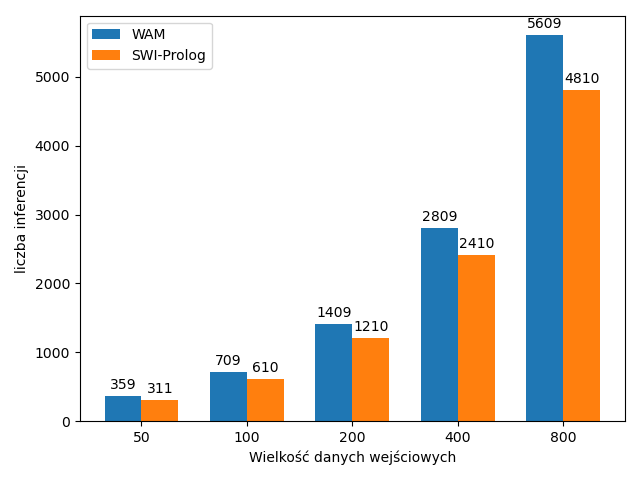
\includegraphics{concati.png}

W przypadku rozcięć liczba inferencji dla proponowanej implementacji i dla SWI-Prologa rośnie liniowo z rozmiarem danych. Dla małych danych SWI-Prolog ma przewagę pod względem liczby inferencji. Przewaga ta też rośnie liniowo.\\

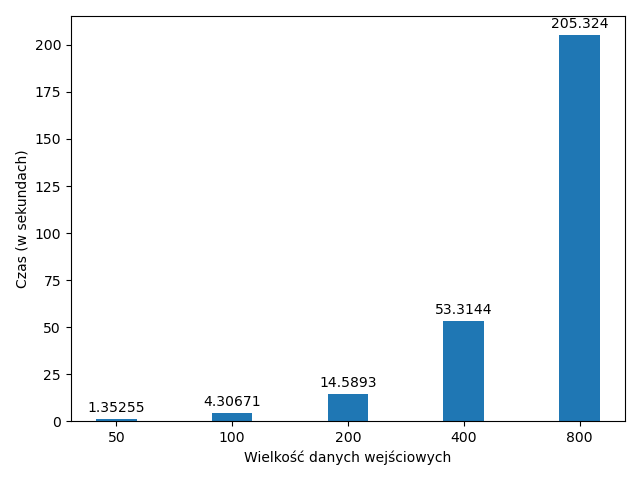
\includegraphics{concattw.png}
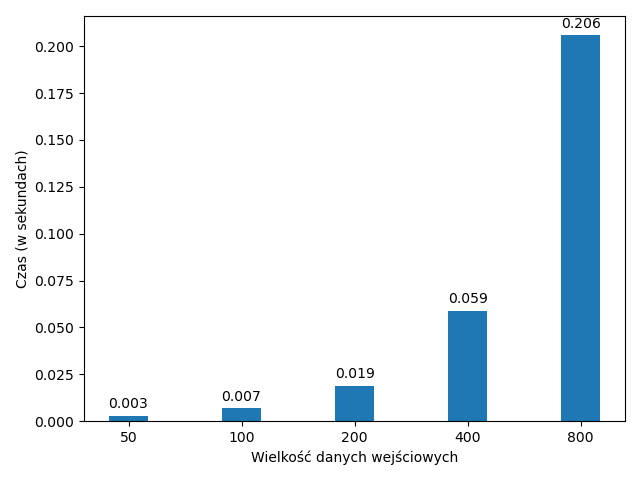
\includegraphics{concatts.png}

Dla pomiarów czasu widać wzrost bliższy kwadratowemu dla obu implementacji, przy czym SWI-Prolog jest około 1000 razy szybszy.

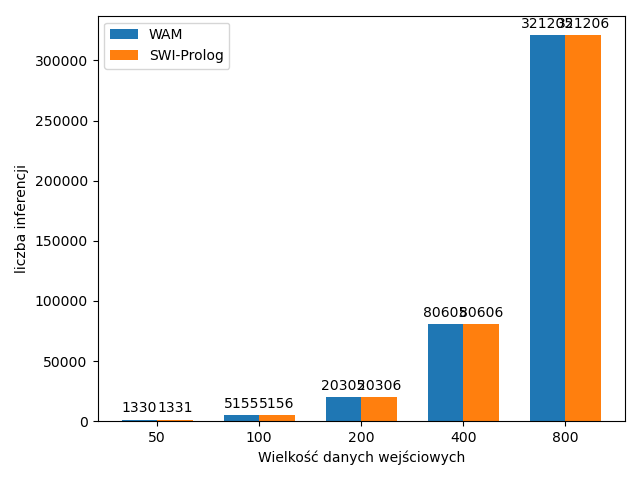
\includegraphics{nrevi.png}

W przypadku naiwenego odwrócenia listy dla dowolnych danych zaproponowana implementacja potrzebuje dokładnie jedną inferencję mniej.

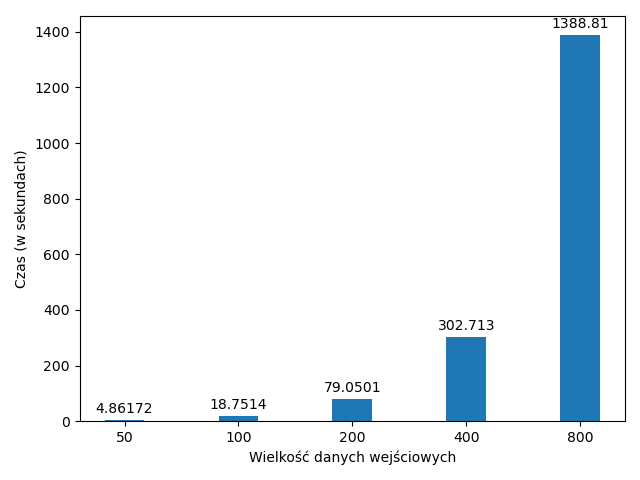
\includegraphics{nrevtw.png}
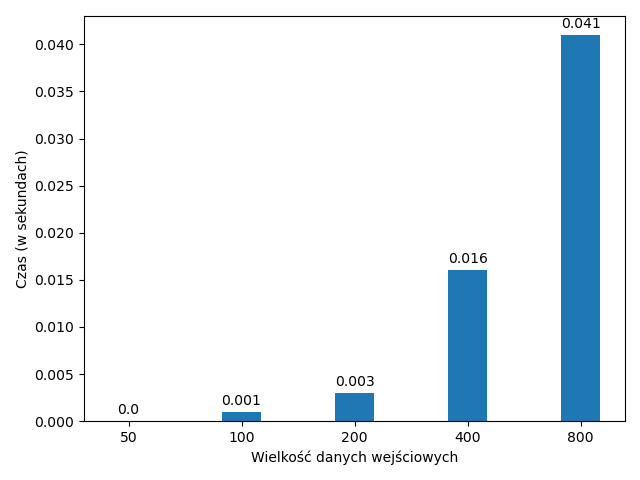
\includegraphics{nrevts.png}

W kategorii czasu dla proponowanej implementacji widać kwadratowy wzrost, to dla SWI-Prologa tempo wzrostu jest trochę mniejsze. SWI-Prolog jest do 33000 razy szybszy.

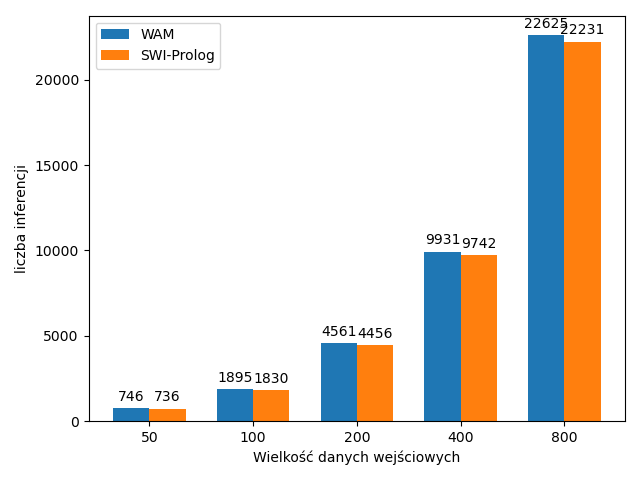
\includegraphics{qsorti.png}

Dla quicksorta różnica w liczbie inferencji tak samo jak dla rozcięć jest na początku niewielka i rośnie ze wzrostem wielkości danych.

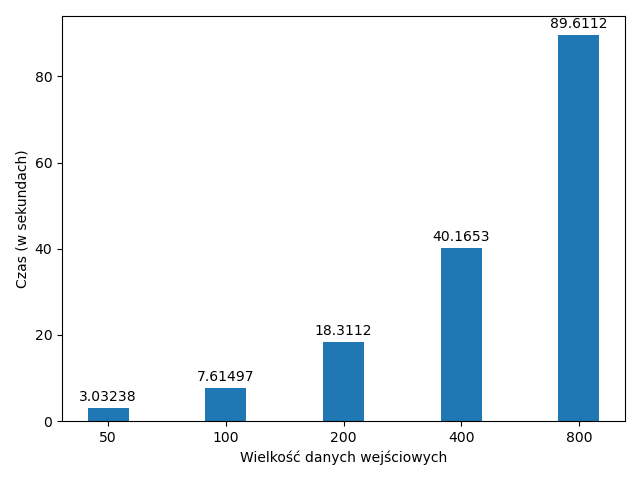
\includegraphics{qsorttw.png}
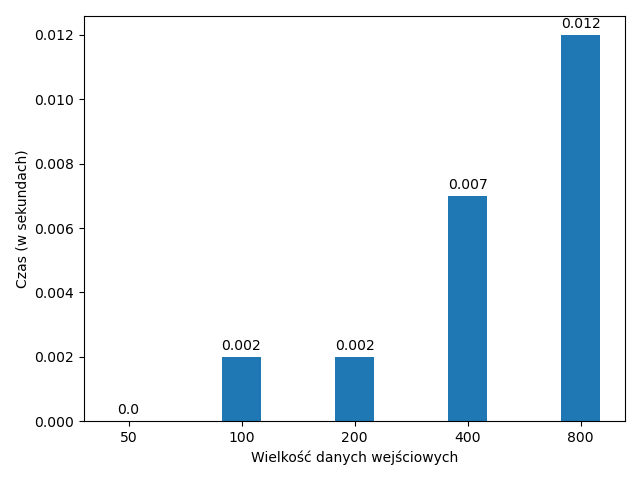
\includegraphics{qsortts.png}

Zależność czasu od wielkości danych jest $O(n\log n)$. SWI-Prolog jest do 7000 razy szybszy.

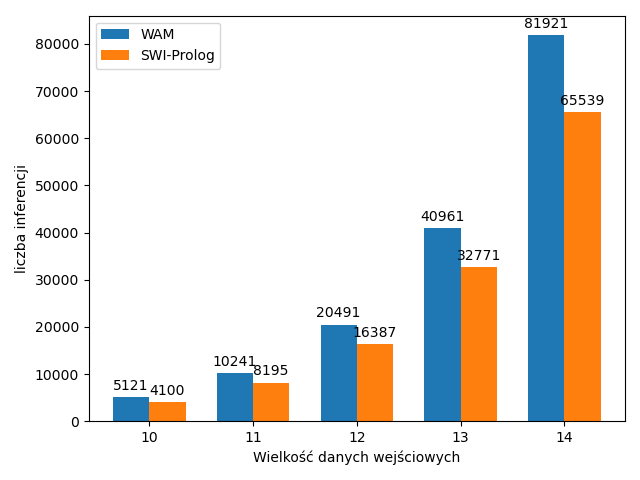
\includegraphics{subsi.png}

W tym wypdaku różnica w liczbie inferencji jest bardziej wyraźna i rośnie wykładniczo.

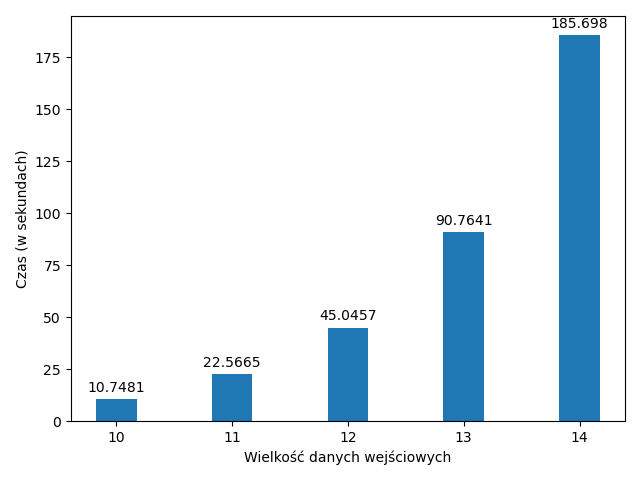
\includegraphics{substw.png}
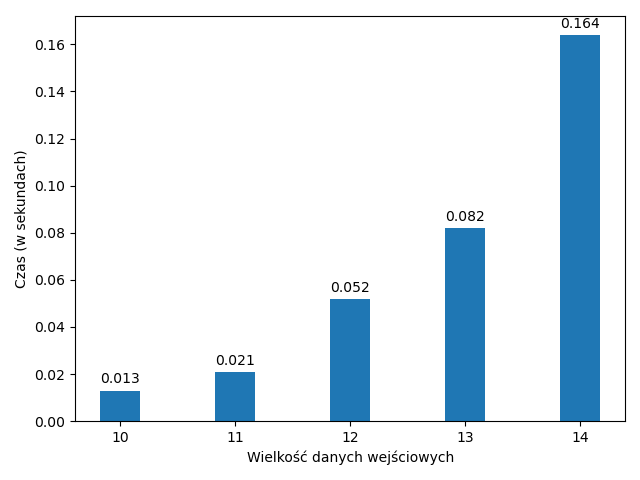
\includegraphics{substs.png}

Potrzebny czas rośnie wykładniczo, a SWI-Prolog jest około 1000 razy szybszy.

